\documentclass{article}
\usepackage[utf8]{inputenc}
\usepackage{graphicx}
\usepackage{enumitem}
\begin{document}
\section{Prihvatanje rezervacija gostiju}
"Prihvatanje rezervacija gostiju" je slučaj upotrebe u kojem se vrši prihvat i obrada digitalnih rezervacija mesta u restoranu. U tom procesu učestvuju potencijalni gost restorana, šef smene/sale restorana, kao i ostali zaposleni.

\begin{itemize}
\item Potencijalni gost restorana posećuje stranicu za digitalne rezervacije i unosi sve potrebne podatke za rezervaciju
\item Šef smene ili sale odobrava rezervaciju na osnovu pregleda prethodno unetih rezervacija i potvrdjuje(ili odbija) rezervaciju potencijalnom gostu.
\end{itemize}
\vspace{1cm}
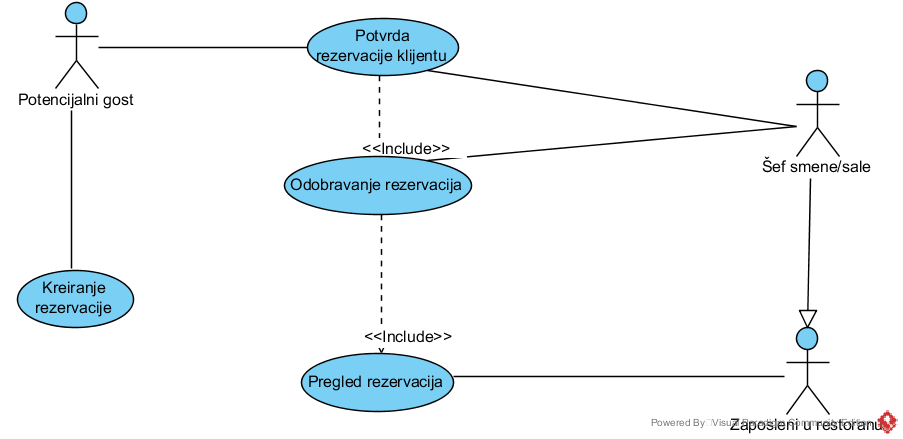
\includegraphics[width=\textwidth]{PrihvatanjeRezervacijaGostiju.png}

\subsection{\textbf{Use Case}: Kreiranje rezervacije}
\textbf{Akter:} Potencijalni gost restorana\\
\textbf{Ulaz:} Kontakt podaci potencijalnog gosta (ime, prezime, kontakt telefon ili e-mail adresa), datum rezervacije, broj gostiju, specijalne napomene\\
\textbf{Izlaz:} Redni broj zahteva za rezervaciju.\\
\textbf{Preduslovi:} Nema.\\
\textbf{Postuslov:} Uspešno je kreiran zahtev za rezervaciju.\\
\textbf{Glavni tok:} Potencijalni gost vrši navigaciju na stranu za rezervaciju, unosi zahtevane podatke i dobija potvrdu da je zahtev za rezervaciju dostavljen restoranu na obradu.\\
\textbf{Alternativni tok:} Potvrda o poslatom zahtevu ne stiže u roku od 2 minuta, prikazuje se izvinjenje i kontakt telefon kojim se može izvršiti rezervacija "offline".\\

\subsection{\textbf{Use Case}: Pregled rezervacija}
\textbf{Akter:} Zaposleni restorana\\
\textbf{Ulaz:} Datum i/ili broj stola za koji se pregleda spisak rezervacija.\\
\textbf{Izlaz:} Spisak registrovanih rezervacija koje odgovaraju kriterijumu pretrage.\\
\textbf{Preduslovi:} Zaposleni ima pristup glavnom sistemu.\\
\textbf{Postuslov:} Nema.\\
\textbf{Glavni tok:} Zaposleni unosi ulazne parametre i dobija tabelarni prikaz registrovanih rezervacija koje zadovoljavaju kriterijume pretrage.\\
\textbf{Alternativni tok:} Nema.\\

\subsection{\textbf{Use Case}:  Odobravanje rezervacija}
\textbf{Akter:} Šef smene/sale\\
\textbf{Ulaz:} Podaci iz pristiglog zahteva za rezervaciju, informacije o već registrovanim rezervacijama i raspoloživom broju i strukturi mesta.\\
\textbf{Izlaz:} Rezervacija odobrena ili odbijena i redni broj rezervacije.\\
\textbf{Preduslovi:} Postoji barem jedan neobradjen zahtev za rezervaciju i trenutni korisnik sistema ima pravo da pristupi odobravanju rezervacija.\\
\textbf{Postuslov:} Informacije o odobrenim rezervacijama su sačuvane u sistemu.\\
\textbf{Glavni tok:} Šef smene/sale pregleda spisak dospelih zahteva za rezervaciju i za svaki od zahteva vrši pregled rezervacija da bi utvrdio da li je rezervacija sa zadatim parametrima moguća, a zatim odobrava ili odbija rezervaciju i svoju odluku registruje u sistemu.\\
\textbf{Alternativni tok:} Nema.\\

\subsection{\textbf{Use Case}: Uklanjanje registrovanih rezervacija}
\textbf{Akter:} Šef smene/sale\\
\textbf{Ulaz:} Redni broj rezervacija koju treba obrisati i razlog brisanja.\\
\textbf{Izlaz:} Nema.\\
\textbf{Preduslovi:} Trenutni korisnik ima pravo da pristupi meniju za uklanjanje registrovanih rezervacija. Postoji validan razlog za uklanjanje rezervacije koji je iskomuniciran sa klijentom (sa čije god strane da je razlog potekao).\\
\textbf{Postuslov:} Rezervacija sa datim rednim brojem je uklonjena iz sistema i razlog uklanjanja je registrovan.\\
\textbf{Glavni tok:} Šef smene/sale unosi ulazne podatke, rezervacija se uklanja iz sistema i korisniku se prikazuju preostale rezervacije za dan uklonjene rezervacije.\\
\textbf{Alternativni tok:} Rezervacija sa datim rednim brojem ne postoji u sistemu. Korisniku se prijavljuje greška i prikazuje se spisak poslednjih deset uklonjenih rezervacija.\\

\subsection{\textbf{Use Case}: Potvrda rezervacije klijentu}
\textbf{Akter:} Šef smene/sale, potencijalni gost restorana.\\
\textbf{Ulaz:} Redni broj rezervacije i kontakt podaci potencijalnog gosta.\\
\textbf{Izlaz:} Rezervacija je potvrdjena ili ne.\\
\textbf{Preduslovi:} Trenutni korisnik ima pravo da pristupi meniju za potvrdjivanje rezervacija, kontakt podaci potencijalnog gosta su validni.\\
\textbf{Postuslov:} Rezervacija je potvrdjena.\\
\textbf{Glavni tok:} Šef smene/sale pregleda odabranu rezervaciju, šalje potvrdu gostu automatski generisanom elektronskom poštom ili poziva gosta telefonom.\\
\textbf{Alternativni tok:} Kontakt podaci nisu validni, rezervacija se automatski registruje kao uklonjena, sa razlogom "nevalidni kontakt podaci gosta".\\ \\

\end{document}